\documentclass[11pt]{article}
\usepackage{amsmath, amssymb}
\usepackage{geometry}
\usepackage{graphicx}
\usepackage{booktabs}
\usepackage{xcolor}
\definecolor{topological}{HTML}{1f77b4}
\definecolor{trivial}{HTML}{d62728}
\geometry{margin=2.5cm}
\graphicspath{{../plots/}}

\newcommand{\Oedge}{X_0 Z_1\cdots Z_{L-2} X_{L-1}}
\newcommand{\expv}[1]{\langle #1\rangle}
\newcommand{\Pop}{\hat{P}}
\newcommand{\code}[1]{\texttt{#1}}

\title{Physical errors in the Kitaev chain:\\ which ones destroy the topological phase?}
\author{Majorana Modes in the Machine}
\date{\today}

\begin{document}
\maketitle

\begin{abstract}
Prof.\ Rosenow's question about the ``usability of Majoranas for quantum
computing,'' made precise: take the \emph{physical} error processes of the Kitaev
chain, translate each through the Jordan--Wigner (JW) map into an operator on our
qubit simulation, and decide which ones actually kill the topological phase. The
organising principle is \textbf{symmetry versus topology}: a perturbation is
harmless only if it is (i) local, (ii) fermion-parity preserving, and (iii)
weaker than the bulk gap $\Delta$. We back this with two exact numerical controls
built on the machinery we already have --- a \emph{robust} error (local
chemical-potential disorder, free-fermion BdG, exact to large $L$) and a
\emph{fatal} one (quasiparticle poisoning, exact diagonalisation so parity can
change).
\end{abstract}

\section{Setup: the Hamiltonian and its three diagnostics}
Under JW the Kitaev chain is the qubit Hamiltonian
\begin{equation}
  H = -\frac{\mu}{2}\sum_j Z_j
      + \frac{t-\Delta}{2}\sum_j X_jX_{j+1}
      + \frac{t+\Delta}{2}\sum_j Y_jY_{j+1},
  \qquad \Pop=\prod_j Z_j,
\end{equation}
topological for $|\mu|<2t$. The logical bit is stored non-locally in the two end
Majoranas $\gamma_L,\gamma_R$ fused into one fermion $f=\tfrac12(\gamma_L+i\gamma_R)$;
its occupation is the fermion parity. Three circuit-measurable objects diagnose it
(all already computed in Blocks~2--4):
\begin{itemize}
  \item the non-local \textbf{string order} $O_{\mathrm{edge}}=\Oedge$ (nonzero in
        the topological phase, zero in the trivial one);
  \item the \textbf{fermion parity} $\Pop=\prod_j Z_j$ (the logical quantum number);
  \item the \textbf{splitting} $\delta E=|E_{\mathrm{even}}-E_{\mathrm{odd}}|\sim
        e^{-L/\xi}$ (the residual overlap of the two Majoranas).
\end{itemize}

\section{The error dictionary}
\begin{center}
\renewcommand{\arraystretch}{1.35}
\begin{tabular}{@{}p{4.6cm}p{5.2cm}p{4.4cm}@{}}
\toprule
\textbf{Physical error (Kitaev $H$)} & \textbf{JW $\to$ qubit operator} & \textbf{Verdict} \\
\midrule
Local potential / charge noise $\delta\mu_i\,c_i^\dagger c_i$ &
$\sum_i\delta h_i Z_i$ \; (local, parity-\emph{even}) &
\textcolor{topological}{\textbf{ROBUST}} up to $\delta h\!\sim\!\Delta$ \\
Zeeman / pairing fluctuation &
local $X_iX_{i+1},\,Y_iY_{i+1}$ (parity-even) &
robust unless it closes $\Delta$ \\
\textbf{Quasiparticle poisoning} $c_i^\dagger$ (a stray electron) &
$\bigl(\prod_{k<i}Z_k\bigr)(X_i\mp iY_i)$ \; (parity-\emph{odd} string) &
\textcolor{trivial}{\textbf{FATAL}}: flips the logical bit, any $L$ \\
Bulk gap closure $\mu\to 2t$ (or strong disorder) &
transverse $\sum_i Z_i$ dominates $\sum_i X_iX_{i+1}$ &
\textcolor{trivial}{\textbf{FATAL}}: topological$\to$trivial transition \\
\bottomrule
\end{tabular}
\end{center}

\noindent The pattern: \textbf{parity-even, sub-gap, local} perturbations are only
virtual excursions across the bulk gap and cannot change the non-local logical
state; \textbf{parity-odd} operators (a single $c_i^\dagger$ --- a JW string ending
in $X/Y$) directly flip it, and \textbf{gap-closing} drives cannot be undone
because the protection itself is gone.

\section{Positive control: local disorder is robust (exact, large $L$)}
Local chemical-potential disorder is charge noise: $\mu\to\mu_j=\mu_0+\delta\mu_j$,
i.e.\ a random parity-preserving field $\sum_j\delta h_j Z_j$. We take
$\delta\mu_j\sim U[-W,W]$ and, using the free-fermion BdG solver generalised to a
\emph{per-site} $\mu_j$ (\code{src/free\_fermion.py}), average $|\expv{O_{\mathrm{edge}}}|$
and the parity gap over disorder realisations, exactly and at large $L$
(\code{src/block4\_errors.py}, \code{disorder\_sweep}). We work at the
representative topological point $\mu_0=t$ (bulk gap $\Delta=2t-\mu_0=t$), chosen
because at $\mu_0=0.5t$ the clean parity gap $\sim(\mu_0/2t)^L$ underflows double
precision by $L\!\sim\!30$ and the edge-Majorana pairing becomes numerically
ambiguous.

\begin{figure}[h]
\centering
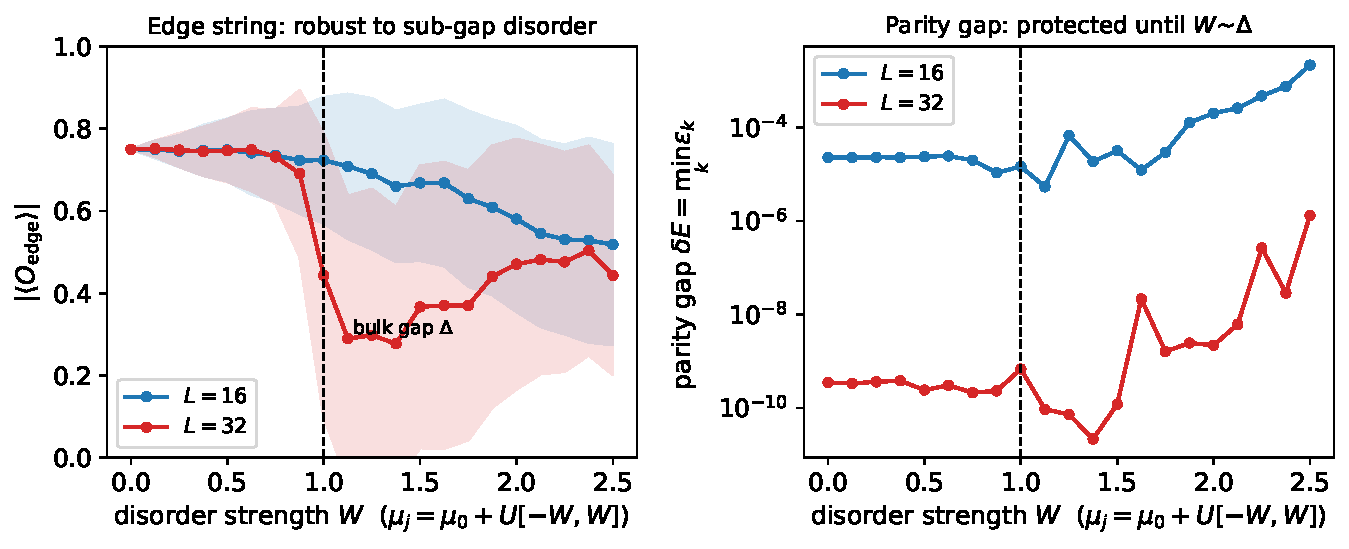
\includegraphics[width=0.95\textwidth]{block4_disorder_robustness.pdf}
\caption{\textbf{Robust error.} Disorder-averaged edge string (left) and parity gap
(right) versus disorder strength $W$, exact to $L=32$. Both are essentially
untouched while $W$ is below the bulk gap $\Delta$ (dashed) and only then degrade:
local, parity-preserving noise is topologically harmless until it approaches the
gap. The splitting is \emph{exponentially smaller} for larger $L$ (right panel),
both curves staying pinned until $W\!\sim\!\Delta$.}
\end{figure}

\section{Negative control: quasiparticle poisoning is fatal (exact diagonalisation)}
A quasiparticle-poisoning event adds or removes one fermion at the end,
$c_0+c_0^\dagger=\gamma_0=X_0$ --- a \emph{parity-odd} boundary operator. Because
the logical bit lives in two \emph{zero-energy} Majoranas, an arbitrarily weak
parity-breaking coupling $g\,X_0$ mixes the near-degenerate even/odd sectors and
destroys it. This is invisible to the (parity-fixed) BdG solver, so we use exact
diagonalisation of the $2^L$ Hamiltonian (\code{contrast\_ed}), contrasting it on
the same chain against the robust parity-preserving $Z$-disorder.

\begin{figure}[h]
\centering
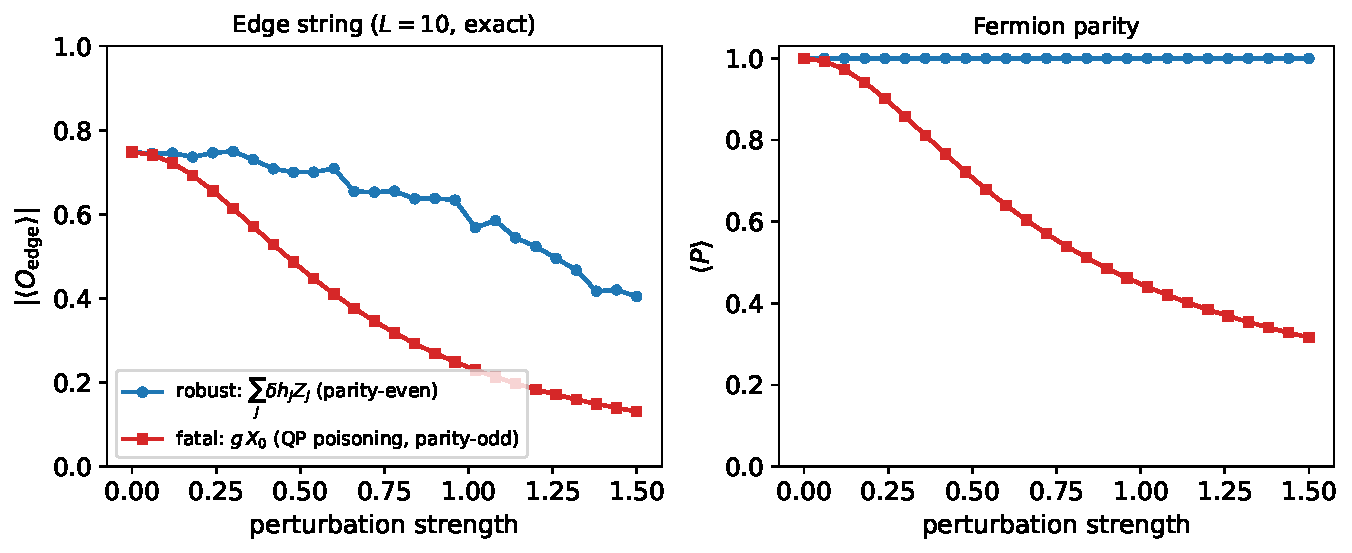
\includegraphics[width=0.95\textwidth]{block4_robust_vs_fatal.pdf}
\caption{\textbf{Robust vs fatal}, same $L$, exact. \textcolor{topological}{Blue}:
parity-preserving $\sum_j\delta h_j Z_j$ keeps $\expv{\Pop}=+1$ and the edge string
near its topological value. \textcolor{trivial}{Red}: the parity-odd
quasiparticle term $g\,X_0$ collapses \emph{both} the parity and the edge string
with no protective threshold. Topological protection is protection against local,
parity-preserving, sub-gap noise \emph{only}.}
\end{figure}

\section{Conclusion --- the usability statement}
Majorana qubits trade the analog fragility of a transmon for a discrete
vulnerability: they are genuinely immune to the local charge and field noise that
plagues conventional qubits (our disorder control), but they inherit \emph{no}
protection against fermion-parity violation. Quasiparticle poisoning is therefore
\emph{the} engineering problem for topological quantum computing --- the poisoning
time must exceed the gate time --- and gap-closing drift ends the protection
outright. This is exactly why our Block-4 result that ``parity (symmetry) is
protected but the edge string (topology) is not noise-immune at fixed $L$'' is the
right lens: symmetry protects the quantum number, topology only protects it
against the errors that respect the symmetry.

\end{document}
